% This work is the property of Aleksandr Salo,
% Student of Baylor University, Computer Science Department. 
% Copying or using without notifying me is not allowed. 
% Contact email is alexsalovrn@gmail.com

\documentclass{article}

\usepackage{fullpage}
\usepackage{url}
\usepackage{hyperref}
\usepackage{amssymb}
\usepackage{amsmath}
\usepackage{graphicx}
\usepackage{epstopdf}
\usepackage{epsfig}
\usepackage{caption}
\usepackage{subcaption}
\usepackage[]{mcode}


\newcommand*{\Perm}[2]{{}^{#1}\!P_{#2}}%
\newcommand*{\Comb}[2]{{}^{#1}C_{#2}}%
\newcommand{\mytilde}{\raise.17ex\hbox{$\scriptstyle\mathtt{\sim}$}}
\newcommand{\patheta}{\frac{\partial}{\partial \theta_j} }
\newcommand{\pathe}{\frac{\partial}{\partial \theta} }
\newcommand{\pathx}{\frac{\partial}{\partial X} }
\newcommand{\thetax}{\theta^T x}
\newcommand{\elll}{\ell(\theta)}
\newcommand{\nath}{\nabla_\theta}
\newcommand{\pelll}{\frac{\partial^2 \elll}{\partial \theta_j \partial \theta_k}}
\newcommand{\ith}{^{(i)}}
\newcommand{\gdafrac}{\frac{1}{(2\pi)^{n/2}|\Sigma|^{1/2}}\exp}

% Dr. Hamerly's customization
% tell Latex to use no paragraph indentation, but leave some space between
% paragraphs 
\setlength{\parindent}{0in}
\setlength{\parskip}{0.1in}

\title{Assignment 4}
\date{Due April 30, 2015}
\author{Aleksandr Salo}

\begin{document}
\maketitle

\section{K-means clustering (20 points)}
	\begin{enumerate}
		\item  \textbf{Number of clusters k}\\
		Given three natural clusters, if we use k = 4 then one cluster inevitably splits on two. Also, mathematically coherently, the cost function decreases with the number of clusters even though they are not good. (Use plotting obj function). 
		\begin{figure}[h]
			\centering
			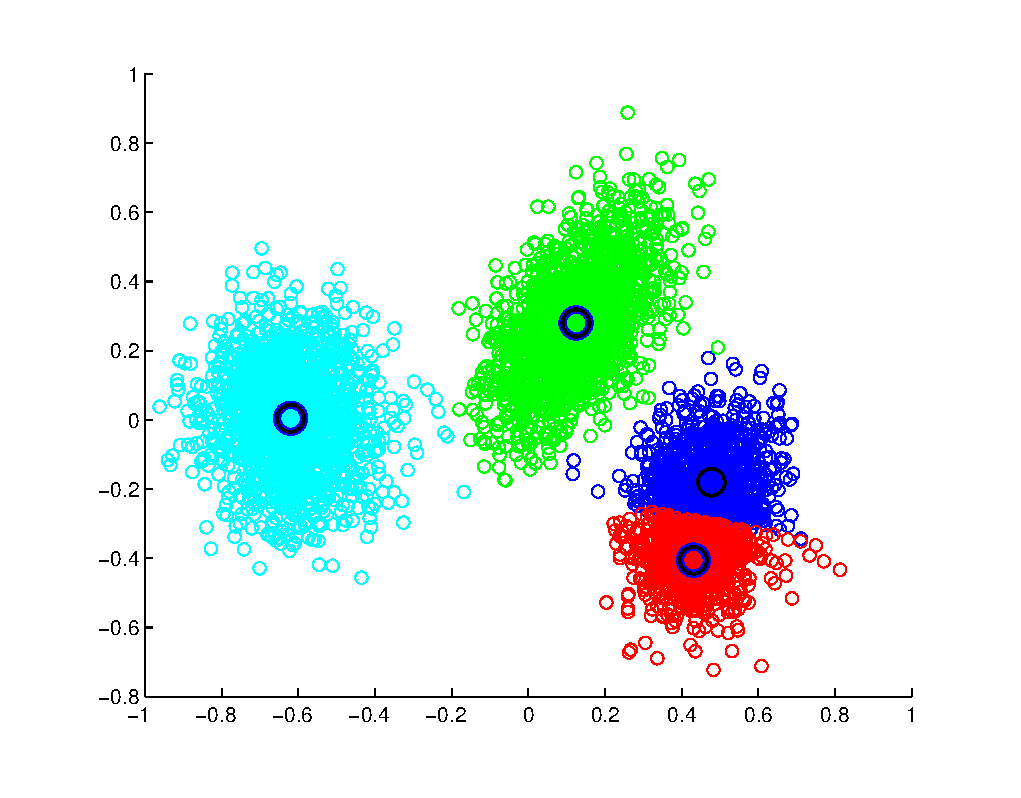
\includegraphics[width=.9\linewidth]{k4_split.eps}
			\caption{Optimal solution, k = 4}
			\label{fig:sub1}
		\end{figure}%
		\pagebreak
		
		\item \textbf{Importance of initialization}\\
		Success of clustering highly depends on the initial guess. Although with given data even random data points assignment to the role of centroids works relatively well, there are common cases when k-mean gets stuck in suboptimal (albeit not necesserilarly bad one) solution.
		
		Given the lucky initialization (with fair chances on this data set) we arrive at seemingly optimal solution.
		
		\begin{figure}[h]
			\centering
			\begin{subfigure}{.6\textwidth}
				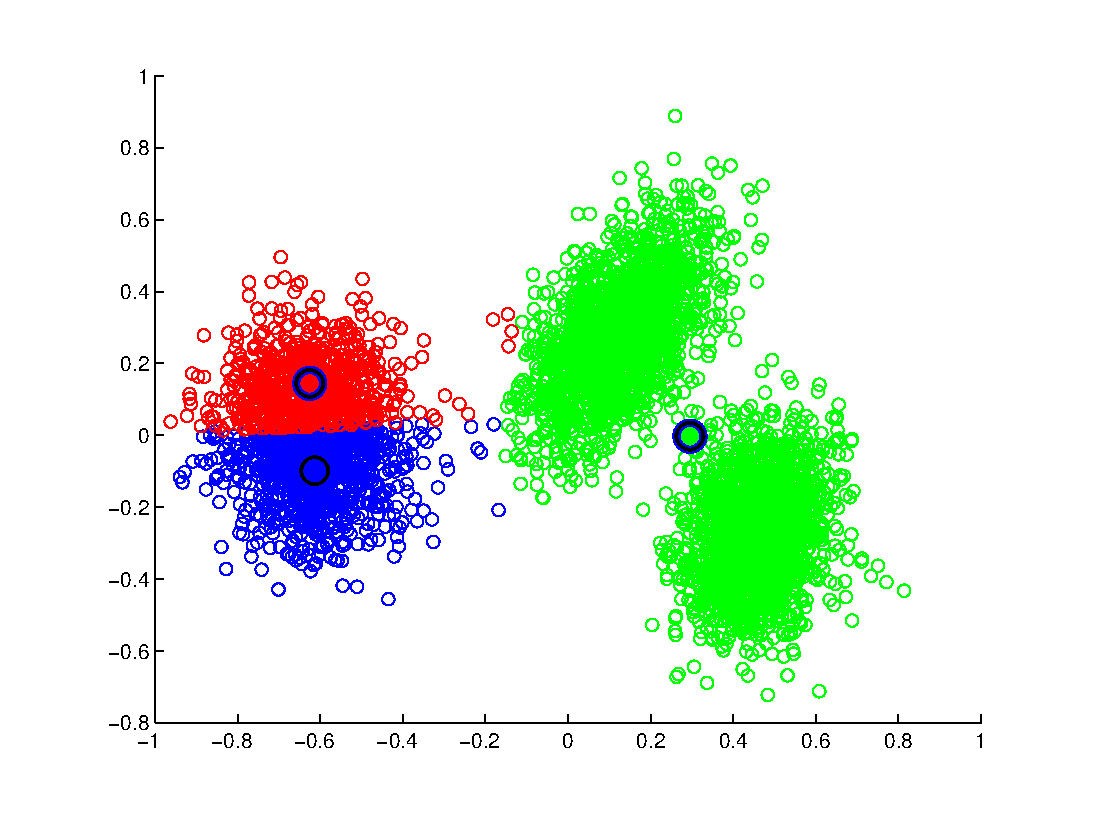
\includegraphics[width=.9\linewidth]{k3_suboptimal_solution.eps}
				\caption{Suboptimal solution, k = 3}
				\label{fig:sub1}
			\end{subfigure}%
			\begin{subfigure}{.6\textwidth}
				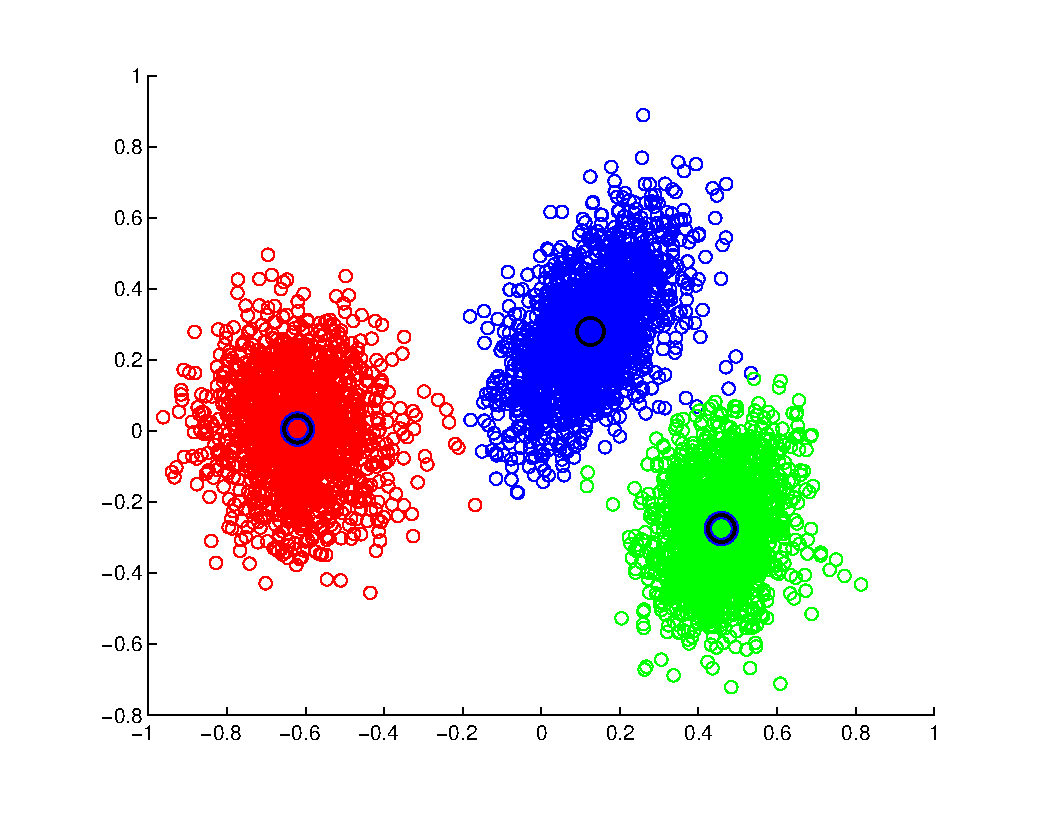
\includegraphics[width=.9\linewidth]{k3_optimal_solution.eps}
				\caption{Optimal solution, k = 3}
				\label{fig:sub1}
			\end{subfigure}
		\end{figure}		
		

		
		
		\item \textbf{How to determine the optimal number of clusters k?}\\
		That is one of the biggest drawbacks for using k-means - that you need to define it yourself. However, we can plot the average value of cost function as a function of number of clusters k. Logically, cost is decreasing with the increase of k. However, at some point making more clusters should not make much of the improvement (if there are some natural clusters). We want to find that sweet spot that likely to indicate the optimal number of clusters.
		
		\begin{figure}[h]
			\centering
			\begin{subfigure}{.6\textwidth}
				\includegraphics[width=.9\linewidth]{errobar_k_rough.eps}
				\caption{Cost function as function of k, rough descent}
				\label{fig:sub1}
			\end{subfigure}%
			\begin{subfigure}{.52\textwidth}
				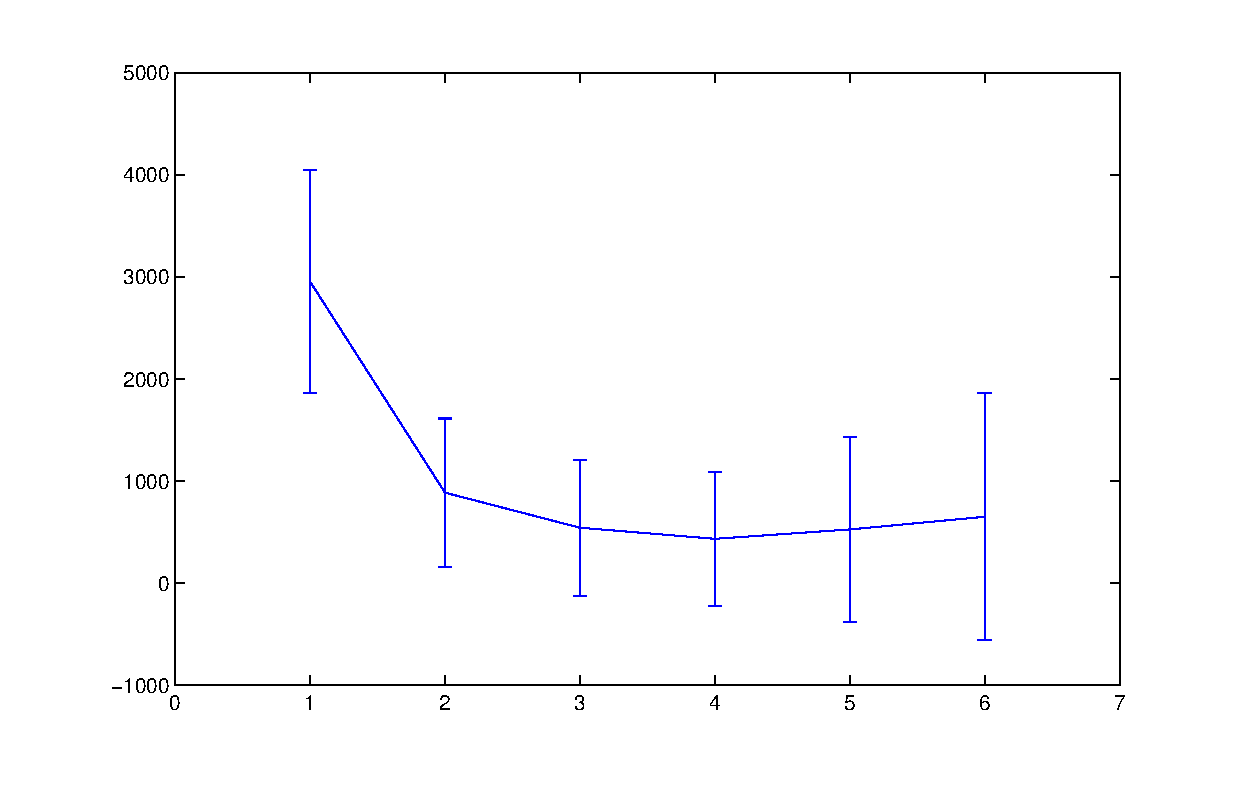
\includegraphics[width=.9\linewidth]{errobar_k_smooth.eps}
				\caption{Cost function as function of k, soft descent}
				\label{fig:sub1}
			\end{subfigure}
		\end{figure}

		Thus we can conclude that the \textbf{optimal k = 3}, which is coherent with our observation of the data.
		However, we need to bear in mind that different initialization could lead to different results thus the plots could look very different and yield slightly different results. Plots above a made with 5 runs for each value of k.  
		
		\pagebreak
		\item \textbf{Convergence}. \\
		I used $J > J_{prev} - \epsilon_{convergence}$ stopping condition, where $\epsilon_{convergence} = 0.1$.\\
		Empirically, more clusters we have - more steps it takes to converge. Visually:
		\begin{figure}[h]
			\centering
			\begin{subfigure}{.6\textwidth}
				\includegraphics[width=.9\linewidth]{convergence_random_init_15runs.eps}
				\caption{Number of steps to converge, random initialization}
				\label{fig:sub1}
			\end{subfigure}%
			\begin{subfigure}{.6\textwidth}
				\includegraphics[width=.9\linewidth]{convergence_smart_init_15runs.eps}
				\caption{Number of steps to converge, k-means++ init}
				\label{fig:sub1}
			\end{subfigure}
		\end{figure}
		Seemingly, there is no significant difference between different initialization methods in terms of number of steps to converge. However, standard deviation seem to be smaller in case of k++ init. 
		
		\item \textbf{Gain of J by k-means++ initialization}
		\begin{figure}[h]
			\centering
			\begin{subfigure}{.6\textwidth}
				\includegraphics[width=.9\linewidth]{cost_random_init_15runs.eps}
				\caption{Cost function (15 runs), random initialization}
				\label{fig:sub1}
			\end{subfigure}%
			\begin{subfigure}{.6\textwidth}
				\includegraphics[width=.9\linewidth]{cost_smart_init_15runs.eps}
				\caption{Cost function (15 runs), k-means++ init}
				\label{fig:sub1}
			\end{subfigure}
		\end{figure}
		
		Notably, smart initialization \textit{(k-means++, choosing the farthest point from all the existing centroids)} gives significantly better results in terms of cost function J, especially when k is close to optimal. Cohesively, for k=3, there is no variation in optimized cost using smart init - we always arrive in the optimal solution on the given dataset. 
		
		\pagebreak
		\textbf{K-means Summary}\\
		\begin{enumerate}
			\item Choice of k is of crucial importance. By choosing wrong number of clusters we doom ourself on failure to determine the natural clusters in data. However, optimized cost function will nonetheless yield suboptimal solution that could be of use. This could be especially true, when clusters are not so naturally separable as in the given dataset.
			
			\item To avoid "guessing" the k, one can deploy the analysis of cost function J as a function of k. By analyzing the such plot one can find a "sweet" spot with, hopefully, the natural number of clusters present in the data. Once again, this would be not so easy given complex overlapping dataset. 
			
			\item Initialization of centroids could be of paramount significance. While simple guess among present data points yields satisfactory results, there is a fair probability of getting stuck in suboptimal solution if the guess was unlucky. To fight this problem, one could use:
			\begin{enumerate}
				\item Smart initialization i.e. k-means++, where we choose centroids iteratively as the farthest point from all existing centroids.
				\item Run k-means several times and choose the run with the best J.\\
				i.e. on given dataset, the chance of getting bad guess is seemed to be around 30 percent. Thus running k-means for 10 times would make the chance of getting bad guess on all 10 runs is negligible $0.3^{10} = 0.000006$							
			\end{enumerate}
			First option seems to be a preferable one (execution time wise).
			
			\item Convergence properties of k-means are impressive. No matter how we initialize the centroids we arrive to the optimal (or suboptimal) solution very fast. On given data set we can observe an empirical rule of: number of steps to converge = 1.5k, where k is a number of clusters.  
		\end{enumerate}
\end{enumerate}

\section{The Generalized EM Algorithm (20 points)}

GEM algorithm makes the following M-step:
$$ \theta \leftarrow \theta + \alpha \nabla_\theta \sum_{i=1}^{m} \sum_{z\ith}^{} Q_i(z\ith) 
	log \frac{p(x\ith, z\ith; \theta)}{Q_i(z\ith)} $$
	
\begin{itemize}
	\item[(a)] Prove that the GEM algorithm described above converges. To do this, you should show that the likelihood is monotonically improving, as it does for the EM algorithm i.e., show that $\ell (\theta^{(t+1)}) \ge \ell(\theta^{(t)})$
	
	\textbf{First let us prove that $\ell (\theta^{(t+1)}) \ge \ell(\theta^{(t)})$ for EM.}\\
	Since we know that $\forall Q_i, \forall \theta$:
	$$\ell(\theta) \ge \sum_{i=1}^{m} \sum_{z\ith}^{} Q_i(z\ith) 
	log \frac{p(x\ith, z\ith; \theta)}{Q_i(z\ith)} $$
	
	Then this would hold true for a particular $Q, \theta$:
	$$\ell(\theta^{(t+1)}) \ge \sum_{i=1}^{m} \sum_{z\ith}^{} Q_i(z\ith) 
	log \frac{p(x\ith, z\ith; \theta^{(t+1)})}{Q_i(z\ith)} $$
	
	Now, since we explicitly choose $\theta^{(t+1)}$ as:
	$$ \theta^{(t+1)} = arg \max_{\theta} \sum_{i=1}^{m} \sum_{z\ith}^{} Q_i(z\ith) 
	log \frac{p(x\ith, z\ith; \theta)}{Q_i(z\ith)} $$
	
	Then:
	$$\sum_{i=1}^{m} \sum_{z\ith}^{} Q_i(z\ith) 
	log \frac{p(x\ith, z\ith; \theta^{(t+1)})}{Q_i(z\ith)} \ge
	\sum_{i=1}^{m} \sum_{z\ith}^{} Q_i(z\ith) 
	log \frac{p(x\ith, z\ith; \theta^{(t)})}{Q_i(z\ith)} $$
	
	Lastly, since we specifically chosen $Q_i(z\ith)  = p(z\ith | x \ith; \theta)$ to make make Jensen's inequality to hold with equality, we can conclude that:
	$$	\ell(\theta^{(t)}) = \sum_{i=1}^{m} \sum_{z\ith}^{} Q_i(z\ith) 
	log \frac{p(x\ith, z\ith; \theta^{(t)})}{Q_i(z\ith)} $$
	
	Considering all three steps together, we proven that:
	$$\ell(\theta^{(t+1)}) \ge \ell(\theta^{(t)})$$
	
	\textbf{Now let us prove that that holds for GEM:}\\
	We can apply the same logic, shortly:
	\begin{align*}
	\ell(\theta^{(t+1)})  &\ge 
	\sum_{i=1}^{m} \sum_{z\ith}^{} Q_i(z\ith) 
	log \frac{p(x\ith, z\ith; \theta^{(t+1)})}{Q_i(z\ith)}\\ &\ge
	\sum_{i=1}^{m} \sum_{z\ith}^{} Q_i(z\ith) 
	log \frac{p(x\ith, z\ith; \theta^{(t)})}{Q_i(z\ith)}\\ &= 
	\ell(\theta^{(t)})	
	\end{align*}
	By the argument given in EM case (Jensen's inequality) the first line holds true. By the choice of distribution for $Q$ we made it hold with equality - thus last line is true. \\
	Lastly, our assumption \textit{"where is a learning rate which we assume is chosen small enough such that we do not decrease the objective function when taking this gradient step."} leads to the second line to be true. 
	
	Hence, the likelihood is indeed monotonically improving with each gradient step.
	$$\ell(\theta^{(t+1)}) \ge \ell(\theta^{(t)})$$ 
	
	
	\item[(b)] Instead of using the EM algorithm at all, suppose we just want to apply gradient ascent to maximize
	the log-likelihood directly. In other words, we are trying to maximize the (non-convex) function
	$$\ell(\theta) = \sum_{i=1}^{m} log \sum_{z\ith}^{} p(x\ith, z\ith; \theta)$$
	so we could simply use the update:
	$$ \theta \leftarrow \theta + \alpha \nabla_\theta \sum_{i=1}^{m} log \sum_{z\ith}^{} p(x\ith, z\ith; \theta)$$
	
	First, let's take the partial derivative of $\ell(\theta)$ of the new approach with respect to $\theta_j$:
	\begin{align*}
	\frac{\partial}{\partial \theta_j} \sum_{i=1}^{m} log \sum_{z\ith}^{} p(x\ith, z\ith; \theta) &=
	\sum_{i=1}^{m} \frac{1}
	{\sum_{z\ith}^{}   p(x\ith, z\ith; \theta)}	
	\sum_{z\ith}^{} \frac{\partial}{\partial \theta_j}  p(x\ith, z\ith; \theta)\\ &=
	\sum_{i=1}^{m} \sum_{z\ith}^{} \frac{1}{p(x\ith; \theta)} 
	\frac{\partial}{\partial \theta_j}  p(x\ith, z\ith; \theta)
	\end{align*}
	
	Now let's do the same for GEM:
	$$\frac{\partial}{\partial \theta_j} \sum_{i=1}^{m} \sum_{z\ith}^{} Q_i(z\ith) 
	log \frac{p(x\ith, z\ith; \theta)}{Q_i(z\ith)} 
	= \sum_{i=1}^{m} \sum_{z\ith}^{} \frac{Q_i(z\ith)}{p(x\ith, z\ith; \theta)} 
		\frac{\partial}{\partial \theta_j} p(x\ith, z\ith; \theta)$$
		
	Since we specifically chosen 
	$Q_i(z\ith)  = p(z\ith | x \ith; \theta) = \frac{p(x\ith, z\ith; \theta)}{p(x\ith; \theta)}$ 
	on the E-step of GEM, then by substitution in the previous equation we have:
	$$
	\sum_{i=1}^{m} \sum_{z\ith}^{} \frac{\frac{p(x\ith, z\ith; \theta)}{p(x\ith; \theta)}}{p(x\ith, z\ith; \theta)} 
	\frac{\partial}{\partial \theta_j} p(x\ith, z\ith; \theta)
	= \sum_{i=1}^{m} \sum_{z\ith}^{} \frac{1}{p(x\ith; \theta)} \frac{\partial}{\partial \theta_j} p(x\ith, z\ith; \theta)$$
	
	That is to say we derived exactly the same result as derivative of the log likelihood. \\
	Thus, $ \theta \leftarrow \theta + \alpha \nabla_\theta \sum_{i=1}^{m} log \sum_{z\ith}^{} p(x\ith, z\ith; \theta)$ procedure gives the same update as the GEM algorithm.
	

	
\end{itemize}


	
	
     
\end{document}